Generally neutrons are born at energies on the order of a few MeV, which is several orders of magnitude above thermal energies.
These neutrons than interact with other nuclei in the material, governed by the probability of a particular reaction occurring.
The probability of a nuclear reaction \eqref{eqn:microXS} can be expressed as probable reaction rate (commonly referred to as the microscopic cross section, $\sigma$) for $n$ neutrons traveling with velocity $v$ a distance $dx$ in a material with an atomic density of $N$.
This also gives rise to the macroscopic cross section, $\Sigma=N\sigma$, where the interpretation is the probability per unit path length of the process described by the microscopic cross section.
\begin{align}
	\label{eqn:microXS}
	\sigma \equiv \frac{\text{reaction rate}}{nvNdx}
\end{align}
If the total cross section is known, the mean free path of the neturon can be calculated as $1/\Sigma_\text{tot}$.
In polyethylene the mean free path of a thermal neutron is about \SI{3.7}{\mm}, and will drecrease with the addition of a strongly absorbing material.
In a scattering medium the n, losing energy, until they are eventually arrive at thermal energies. 
In pure hydrogen it takes 27 elastic collisions for a \SI{2}{\MeV} neutron to slow down to \SI{0.025}{\electronvolt}, and 119 collisions in carbon.
The rate of flow of neutrons is described by the neutron flux and is calculated as the neutron density multiplied by the neutron velocity.
The neutron fluence is then the integrated neutron flux over a given rate of time.

They are several nuclear interactions that are of interest for radiation portal monitors, of which several are presented in \autoref{tab:NeutronRxnProducts}.
\begin{table}
	\caption[Neutron Reactions and Reaction Energies]{Typically isotopes used in neutron radiation detectors}
	\label{tab:NeutronRxnProducts}
	\begin{tabular}{ c | c c c} 
		\toprule
		Reaction                           & Q-Value (MeV) & Thermal Cross Section & Application \\
		\midrule
		${}^3He + n \to p +{}^3H$          & 0.756     & 5,330 & Proportional counter gas \\
		${}^6Li + n \to {}^3H + \alpha$    & 4.78      & 940 & Lithium glass scintillators \\
		${}^{10}B + n \to \alpha + {}^7Li$ & 2.31      & 3,840 & Plastic scintillators \\
		${}^{157}Gd + n \to \gamma$        &various    & 259,000 & various \\
		\bottomrule
	\end{tabular}
\end{table}
The dependance of the cross section on the energy of the neutron is shown in \autoref{fig:NeturonXS}.
The desire to thermalize the neutron flux (decreasing the average energy of the neutrons) is evident due to the dramatic increases of the cross sections for lower energies.
\begin{figure}
	\centering
	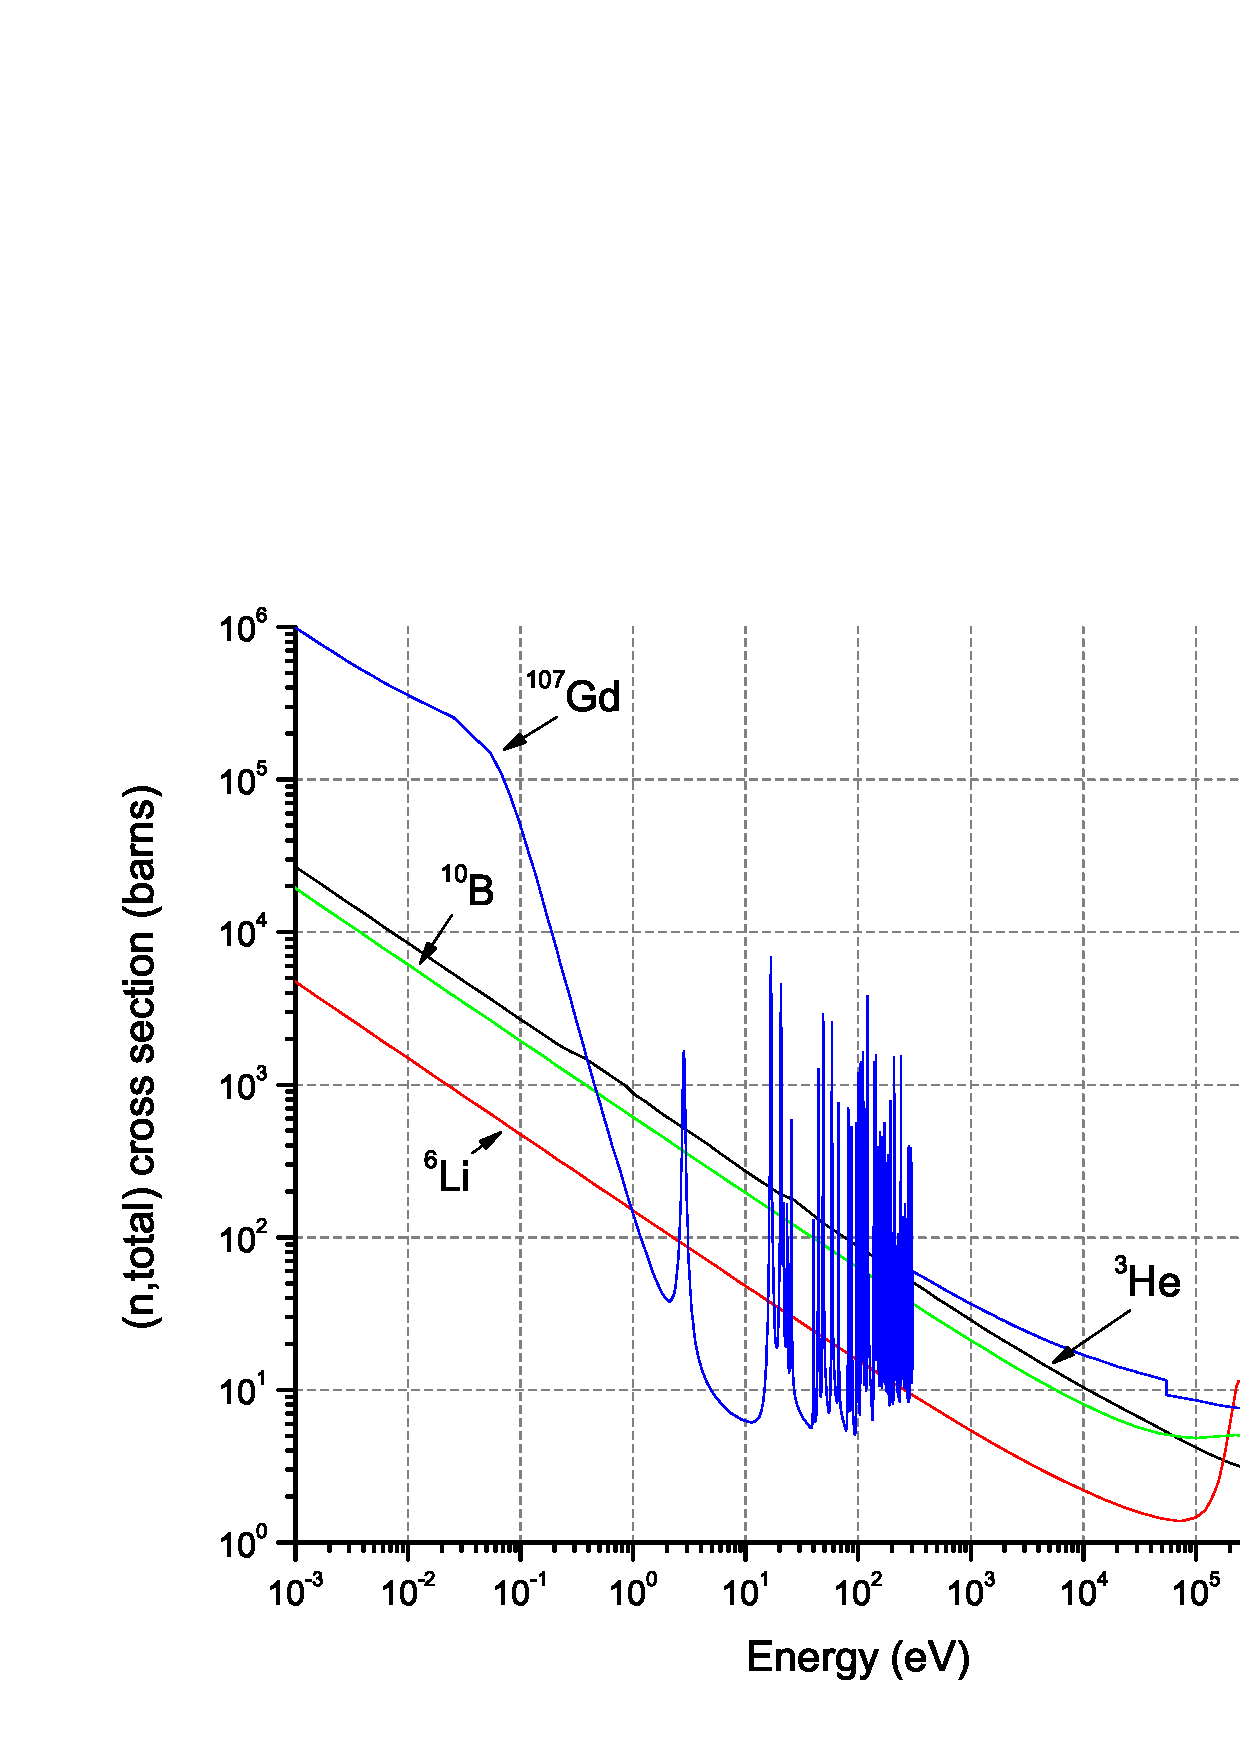
\includegraphics[width=\textwidth]{NeutronXS}
	\caption[Neutron Reaction Cross Sections]{Cross sections of typical isotopes used in neutron radiation detectors.  Neutrons at room temperature have an energy of \SI{0.025}{\eV}.}
	\label{fig:NeutronXS}
\end{figure}
